\documentclass[apj]{emulateapj}
%\usepackage{apjfonts}
\usepackage{graphicx}
\usepackage{amsmath,amssymb}
%\usepackage{Times}
%\usepackage{natbib}
\usepackage{amsmath}

\bibliographystyle{apj}

\def\mnras{MNRAS}
\def\apj{ApJ}
\def\aj{AJ}
\def\apjl{ApJL}
\def\aap{AAp}
\def\nat{Nature}
\def\pasj{PASJ}
\def\jcap{JCAP}
\def\prd{PRD}
\def\pasp{PASP}

\let\oldAA\AA
\renewcommand{\AA}{\text{\normalfont\oldAA}}

\begin{document}

\title{The Supernova Rate Beyond The Optical Radius}

\author{People (Brennan Dell, Sukanya Chakrabarti, Ben Lewis, Or Graur, Alex Filipenko)}

\begin{abstract}
Many spiral galaxies have extended outer HI disks, and display low levels of star formation, inferred from the FUV emission detected by GALEX, well beyond the optical radius. Here, we investigate the supernova rate (SN rate) in the outskirts of galaxies, using the largest and most homogeneous set of nearby supernova from the Lick Observatory Supernova Search (LOSS).    Up to now, supernova rates have been measured with respect to various galaxy properties, such as stellar mass and metallicity, but not with respect to galactocentric radius.  Understanding the SN rate as a function of intra-galactic environment has many ramifications -- from the interpretation of LIGO observations, the formation of massive stars, to the observed high velocity dispersion of the outer HI disk.  Using the data from the LOSS survey, we find that supernovae in dwarf galaxies (with a stellar mass less than $10^{9} M_{\odot}$) host 3.962 +/- 2.175 supernovae per millennium, while supernovae beyond the optical radius of spiral galaxies occur at a rate of 2.480 +/- 0.490 supernovae per millennium. The agreement in these figures suggests that the outskirts of spiral galaxies are just as likely to be hosts of binary black hole mergers as dwarf galaxies are. In the future, better measurements of the stellar mass in the outskirts of galaxies as well as larger homogeneous samples of supernova data should refine this measurement, and clarify the relationship between the supernova rate and galactocentric radius.
\end{abstract}

\section{Introduction}

The rate of supernovae is a fundamental quantity that has far-reaching implications for many areas of astrophysics and cosmology.  The SN rate is directly tied to the metal enrichment of galaxies, and the birth rate of neutron stars and black holes.  Earlier work has assembled a large and homogeneous set of nearby SNe (Leaman et al. 2011), i.e., the LOSS survey, that has been analyzed to search for correlations between the SN rate and galaxy properties (Graur et al. 2017).  Many spiral galaxies have extended HI disks (Walter et al. 2008), and display FUV emission in the outskirts (Thilker et al. 2007; Bigiel et al. 2010) that is indicative of a low level of star formation beyond the optical radius. Some of these stars will explode as supernovae, but the SN rate in the outskirts of galaxies has not yet been determined.  Here, we analyze the LOSS survey to directly determine the SN rate beyond the optical radius.

Recent LIGO observations (Abbott et al. 2016; Abbott et al. 2017) indicate that these merging massive binary black holes form in regions of low metallicity (Belczynski et al. 2016).  Several recent papers have now studied the host galaxies of binary black hole (BBH) mergers with binary merger population synthesis models (Lamberts et al. 2016; O'Shaughnessy et al. 2017; Chakrabarti et al. 2017).  Lamberts et al. (2016) showed that these events are either arising from dwarf galaxies or massive galaxies at high redshift.  O'Shaughnessy et al. (2017) noted that due to the low metallicity star formation found in dwarf galaxies, binary black hole mergers would be abundantly produced there.  Chakrabarti et al. (2017) found that the outskirts of spiral galaxies, which manifest a low level of star formation and have low metallicities, would contribute at least as much to the observed LIGO/Virgo detection rates as dwarf galaxies do.  If this is correct, one may expect that other tracers of the formation of massive stars should also be present in the outer disk, and the SN rate is one such tracer that we investigate here.

A puzzling observation of outer HI disks is that the velocity dispersion close to $R_{25}$ (where the B-band reaches 25-th magnitude) is about 10 km/s, which Tamburro et al. (2009) noted would require an unrealistic amount of supernova feedback efficiency if supernova were entirely responsible to maintaining the velocity dispersion in the outer disk.  Their estimate of the SN rate is however indirect, and is based on the observed star formation rate.  Here, we also investigate this puzzling observation, but with a direct calculation of the supernova rate beyond the optical radius.  

This paper is organized as follows.   In \S 2, we briefly review the parameters of the LOSS survey and summarize how we calculate SN rates here.  In \S 3, we present our main results, and we contrast in particular the SN rate in the outskirts of spiral galaxies with the rate in dwarf galaxies as a whole,  In \S 4, we discuss the ramifications of this result, and we conclude in \S 5.

\section{Methods}

The Lick Observatory Supernova Search (LOSS) has produced the largest homogeneous sample currently available of galaxies used for supernova rate calculation. This sample is magnitude limited to ~19 magnitudes, contains 14,878 galaxies, and hosts 929 supernovae. (Leaman et al. 2010). Galaxies in the sample are grouped by hubble type into eight classes —E, S0, Sa, Sb, Sbc, Sc, Scd, and Irr (irregular), and supernovae are classified as type Ia, SE or II. Leaman et al. (2010) provide data from this survey on the position of the supernovae within their host galaxies, as well as parameters describing the apparent shape of the galactic disks. In addition, Graur et al. (2017) provide control times for the LOSS sample galaxies used in supernova rate calculations. Using these two data sets, rates of supernovae can be calculated for specific regions of a galaxy defined by galactocentric radius. We use this approach to determine the supernova rate in the outskirts (r > R25) of spiral galaxies, and analyze the results.

The data Leaman et al. (2010) collected from the LOSS sample contains the offset coordinates of each supernova from the center of its host, as well as each galaxy’s position angle, major axis length, and minor axis length. The major and minor axes are measured from the ellipse which fits the boundary of the 25th magnitude in the B-band. Using these parameters, the offset vector can be rotated and scaled to produce the vector as it would appear if the host galaxy were viewed face-on. The result is this vector:

*** Vector Equation Here ***

Where x’’ is the right ascension offset, y’’ is the declination offset, PA is the position angle, d1 is the major axis length, and d2 is the minor axis length. Dividing the length of this adjusted vector by the semi-major axis length produces the galactocentric radius of the supernova expressed as a multiple of R25.

*** Length Equation Here***

Although this is a crude method of distance measurement, it is sufficient to determine which supernovae explode beyond the optical radii of galaxies.

The figure below shows the distribution of supernovae vs the galaxy stellar mass:

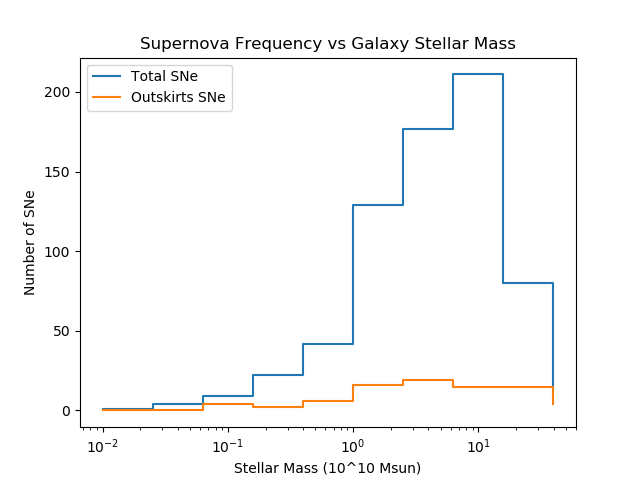
\includegraphics[scale=0.5]{supernova_freq_vs_stellar_mass}

The small number of supernovae in the low mass range is caused by the lack of low mass galaxies in the galaxy sample. As Leaman et al. (2010) mention, this is due to a Malmquist bias in the LOSS sample.

In addition, Graur et al. (2017) provide the control times and stellar masses for each of the galaxies in the LOSS survey. When this data is combined with the parameters from the data gathered by Leaman et al. (2010), supernova rates can be calculated with respect to galactocentric radius.

We calculate supernova rates using the mass-normalized control time method. The specific supernova rate for a sample of galaxies is calculated with this equation.

*** Control-time Equation ***

Where N is the number of supernovae of a certain type in the sample, tci is the control time of the ith galaxy, and M*i is the stellar mass of the ith galaxy (Graur et al. 2017). Calculating the “specific” supernova rate accounts for the fact that the specific supernova rate increases as a galaxy’s stellar mass decreases (Leaman et al. 2010). If the mass of a galaxy is known along with its specific supernova rate, then the number of supernovae per year can be calculated. We choose to represent the specific supernova rates in SNuM units, where 1 SNuM is 10-12 SN yr-1 solar mass-1 (Graur et al. 2017).

The luminosity data used to calculate the stellar masses of the galaxies is not available for all galaxies in the sample. Leaman et al. (2010) avoid this problem by excluding these galaxies from the rate calculations. We use the same approach to calculate our supernova rates. In order to increase the sample size of galaxies for the supernova rate calculation, Graur et al. (2017) extrapolated the galaxy stellar masses using partially available luminosity data. The supernova rates which we defined could be improved using a similar approach.

The control time for a given galaxy varies depending on the type of supernova that is being observed. We calculate the total supernova rate, or the supernova rate regardless of type, as the sum of the rate of each type of supernova:

*** Rate Total Equation ***

Using the data collected by Leaman et al. (2010) and Graur et al. (2017), the supernova rate in the outskirts of spiral galaxies can be calculated using the above equation on a sample of spiral galaxies where N is the number of supernovae occuring beyond R25. Calculating this rate for the outskirts of spiral galaxies can then be compared to the rate of supernovae in dwarf galaxies.

\section{Results}

In the sample of LOSS galaxies, supernovae are found to be distributed like so:

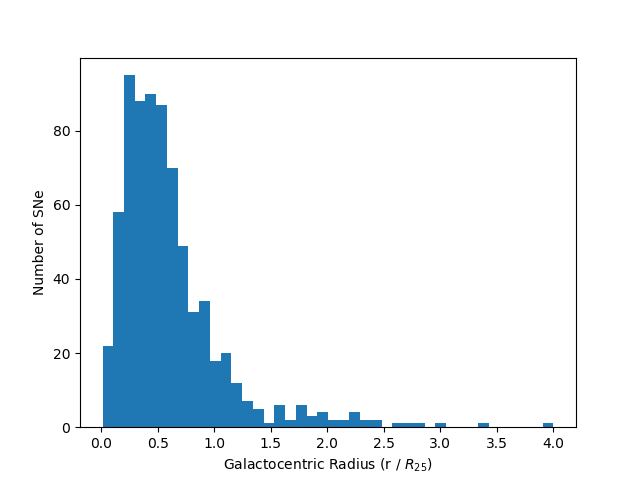
\includegraphics[scale=0.5]{sne_vs_radius}

Leaman et al. (2010) attribute the small number of supernovae near the center of the galaxy to extinction effects from the galactic bulge. Aside from that, the number of supernovae declines as a power law as the galactocentric radius increases. Supernovae can be seen well beyond the optical radius.

The dependence of rate vs. mass was measured to compare it with the supernova rates overall. We attempted to replicate the plot of the specific supernova rate vs. mass in the same manner as Graur et al. (2017).

The plot in red below is produced by grouping galaxies by their stellar mass into bins by their stellar mass, then plotting the rate and the errors for each rate. The sliding bin line in blue is plotted by using the same bin size as the fixed bins, but the bin “slides” along the x-axis, and calculates the supernova rate of the galaxies it contains. The gray shaded region shows the Poisson errors for this calculation. A power law was fit to the fixed bins, and is plotted in green.

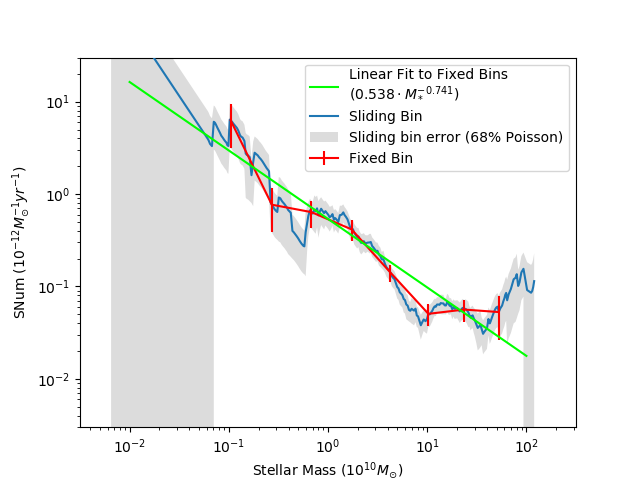
\includegraphics[scale=0.5]{outskirts_sn_rate_vs_mass}

*** SN Rate vs Mass Table ***

Fitting a power law to the fixed bins in this plot produces a specific supernova rate function given a galaxy’s stellar mass:

*** Rate SN Total from Mass Equation ***

Multiplying this specific rate by the galaxy’s stellar mass produces the number of supernovae per year:

*** SNe / year equation ***

To calculate the supernova rate for the outskirts of spiral galaxies, a sample of spiral galaxies was selected from the sample. The size of the sample of spiral galaxies is 8,348 galaxies, which contain 73 supernovae in the outskirts. The mean mass of the sample is 6.959 * 1010 solar masses. The specific supernova rate for all types of supernovae is 0.035 +/- 0.007 SNuM. The error in this rate is the 68\% Poisson uncertainty. Multiplying this specific rate by the mean mass of this sample produces a supernova rate of 2.432 +/- 0.497 SNe per millenium.

The rate for dwarf galaxies was also calculated. The sample of dwarf galaxies was created by selecting all the galaxies with a stellar mass less than 109 solar masses. This selection contains 432 dwarf galaxies, which contain 11 supernovae. The mean mass of a galaxy sample is 4.476 * 108 solar masses. The specific supernova rate for this sample is 8.851 +/- 4.859 SNuM. Multiplying this specific rate by the mean mass of this sample produces a supernova rate of 3.962 +/- 2.175 SNe per millenium.

\section{Discussion}

Although the data from the outskirts of spiral galaxies and especially from dwarf galaxies is very sparse, the broad agreement in these figures provides empirical evidence for the claim that the outskirts of spiral galaxies are just as likely to be a source of binary black hole mergers.

The scarcity of the dwarf galaxies is due to the fact that the LOSS sample is magnitude limited to ~19 magnitudes (Leaman et al. 2010). Leaman et al. (2010) also mention that irregular galaxies are underrepresented in the galaxy sample, which occur most frequently in low mass galaxies (Kelvin et al. 2014).

The direct measurement of the supernova rate beyond the optical radius also provides a direct method of determining the energy input rate of supernova into the extended HI disks of spiral galaxies. Using an estimation of the supernova rate, Tamburro et al. (2009) determine that the supernova feedback efficiency would need to be unrealistically high to account for the observed turbulence in the HI regions in the outskirts of spiral galaxies. This conclusion could be supported directly using the supernova rates which we have derived here.

\section{Conclusion}

This broad agreement suggests that the outskirts of spiral galaxies is a region which deserves closer research. Deeper surveys of these galaxies could provide better information on galactic outskirts, such as star formation rate and stellar mass, which would further elucidate the contribution of spiral outskirts to black hole mergers. 

The measurements of the supernova rate in the outskirts could be improved using samples with a larger and more representative number of dwarf galaxies. In particular, a volume-limited sample would allow the total number of observed supernovae from dwarf galaxies and from spiral galaxy outskirts to be calculated, thus providing a more robust tracer of their contributions to the signal from binary black hole collisions.


This material is based upon work supported by the National Science Foundation under Grant No. 1517488. Any opinions, findings and conclusions or recommendations expressed in this material are those of the authors and do not necessarily reflect the views of the National Science Foundation.

\end{document}
